\documentclass[12pt,a4paper]{article}
\usepackage[a4paper,top=20mm,bottom=20mm,left=25mm,right=15mm]{geometry}
\usepackage[T2A,T1]{fontenc}
\usepackage{indentfirst}
\usepackage[utf8]{inputenc} 
\usepackage[english,russian]{babel}
\usepackage{amsmath}
\usepackage{amssymb}
\usepackage{graphicx}
\usepackage{float}
\usepackage{listings}
\usepackage{xcolor}
\usepackage{hyperref}
\usepackage{siunitx}

\lstset{
    language=C++,                
    basicstyle=\ttfamily\small,   % Шрифт
    keywordstyle=\color{blue},    % Цвет ключевых слов
    commentstyle=\color{gray},    % Цвет комментариев
    stringstyle=\color{orange},   % Цвет строк
    numbers=left,                 % Нумерация строк
    numberstyle=\tiny\color{gray},% Стиль нумерации
    stepnumber=1,                 % Каждая строка нумеруется
    numbersep=5pt,                % Отступ номеров от кода
    backgroundcolor=\color{white},% Фон
    showspaces=false,             % Не показывать пробелы
    showstringspaces=false,       % Не показывать пробелы в строках
    showtabs=false,               % Не показывать табуляцию
    frame=single,                 % Рамка вокруг кода
    breaklines=true,              % Перенос строк
    breakatwhitespace=false,      % Перенос по пробелам
    tabsize=2                     % Размер табуляции
}
\begin{document}

\begin{center} 
МИНИСТЕРСТВО ОБРАЗОВАНИЯ И НАУКИ РОССИЙСКОЙ ФЕДЕРАЦИИ \\
Федеральное государственное автономное образовательное учреждение  \\
высшего образования\\ \textbf{<<Национальный исследовательский \\ Нижегородский государственный университет \\
им. Н.И. Лобачевского>>}\\
\textbf{(ННГУ)}\\[0.5cm]
\textbf{Институт информационных технологий, математики и механики}\\[4.5cm]

\textbf{\large Отчет по лабораторной работе} \\[0.6cm]
\textbf{Тема:}\\
  \textbf{\large <<Построение выпуклой оболочки – проход Джарвиса>>}\\[3.0cm]
\begin{flushright}
 \begin{minipage}{0.40\textwidth}
 \begin{flushleft}
  \textbf{Выполнил:}\\[0.1cm]
  студент группы 3822Б1ФИ1 \\
  Шульпин Илья Евгеньевич  \\[1.0cm]
  \textbf{Преподаватели:}\\[0.1cm]
  Сысоев Александр Владимирович, доцент, кандидат технических наук  \\[0.1cm]
  Нестеров Александр Юрьевич, аспирант  \\[0.1cm]
  Оболенский Арсений Андреевич, преподаватель  \\
 \end{flushleft}
 \end{minipage}
\end{flushright}
 \vfill 

  Нижний Новгород \\
 2025

 \thispagestyle{empty} 

\end{center}

\newpage
\section{Введение}

Задача построения выпуклой оболочки является одной из фундаментальных в вычислительной геометрии и находит применение в задачах распознавания образов, компьютерной графике, анализе данных и геоинформационных системах. Пусть задано множество точек 
\[
S = \{\,p_1, p_2, \dots, p_n\} \subset \mathbb{R}^2.
\]
Выпуклой оболочкой множества $S$ называется наименьшее по включению выпуклое множество, содержащее $S$. Формально:
\[
\mathrm{Conv}(S) = \bigcap_{\substack{{C \subset \mathbb{R}^2}\\{C\text{ — выпуклое}}}} \{\,C \mid S \subset C\}.
\]

Одним из классических алгоритмов построения выпуклой оболочки называется метод «обёртывания подарка» или «проход Джарвиса» (Jarvis March). Идея алгоритма заключается в следующем:
\begin{enumerate}
  \item Находим точку $p_0$ с наименьшей абсциссой (или крайнюю слева): 
    \[
      p_0 = \arg\min_{p\in S} x(p).
    \]
  \item С текущей граничной точкой $p_i$ ищем такую точку $p_{i+1}$, что все остальные точки множества $S$ лежат по левую сторону от направленного вектора $\overrightarrow{p_i p_{i+1}}$. Это эквивалентно максимизации поворотного угла:
    \[
      p_{i+1} = \arg\min_{p \in S \setminus \{p_i\}}
                  \Bigl(\, \angle (\overrightarrow{p_{i-1}p_i}, \overrightarrow{p_i p}) \Bigr).
    \]
  \item Повторяем шаг 2 до тех пор, пока вновь выбранная точка не совпадёт с $p_0$.
\end{enumerate}

Алгоритмическая сложность метода Джарвиса составляет
\[
  O(n \cdot h),
\]
где $n = |S|$ — общее число точек, а $h$ — число точек на самой выпуклой оболочке. В худшем случае ($h = n$) сложность вырождается в $O(n^2)$, однако на «узких» оболочках (когда $h \ll n$) алгоритм работает значительно быстрее.

В данной работе предлагаются и сравниваются следующие реализации алгоритма Джарвиса:
\begin{itemize}
  \item классическая последовательная версия;
  \item параллельные версии, реализованные с использованием OpenMP, Intel TBB, параллельных возможностей STL и гибридного подхода MPI + Parallel STL.
\end{itemize}

\section{Постановка задачи}
Необходимо исследовать алгоритм Джарвиса (Jarvis March) для построения выпуклой оболочки множества точек в $\mathbb{R}^2$, реализовать его в последовательном и параллельных вариантах, а также выполнить сравнительный анализ их эффективности.

\subsection*{Цель работы}
\begin{itemize}
    \item Разработка, реализация и экспериментальное исследование алгоритма Джарвиса для построения выпуклой оболочки в последовательном и параллельных режимах.
\end{itemize}

\subsection*{Задачи работы}
\begin{itemize}
    \item Спроектировать и реализовать \textbf{последовательную} версию алгоритма Джарвиса.
    \item Разработать \textbf{параллельные} реализации алгоритма с использованием:
    \begin{itemize}
        \item OpenMP;
        \item Intel TBB (oneAPI TBB);
        \item Стандартные потоки C++ (`std::thread`);;
        \item гибридного подхода MPI + std::thread
    \end{itemize}
    \item Проверить корректность всех реализаций на наборе тестовых данных.
    \item Провести сравнительный анализ производительности (время выполнения, масштабируемость) последовательной и параллельных реализаций.
    \item Оценить влияние числа потоков / процессов и размеров входного множества на эффективность алгоритма.
\end{itemize}

\section{Язык программирования}

Для реализации проекта выбран язык C++ благодаря его высокой производительности, эффективному управлению памятью и возможности низкоуровневого доступа к аппаратному обеспечению. Современные стандарты C++17/20 предоставляют встроенные средства распараллеливания, а экосистема дополняется следующими инструментами:

\begin{itemize}
  \item \textbf{std::thread} — низкоуровневая библиотека потоков из стандартной библиотеки C++ для создания и управления потоками вручную;
  \item \textbf{OpenMP} — директивная модель многопоточности с лаконичным синтаксисом и широкой поддержкой компиляторов;
  \item \textbf{Intel oneAPI Threading Building Blocks (TBB)} — библиотека для гибкого построения задачно-ориентированных параллельных графов;
  \item \textbf{MPI} — интерфейс для организации распределённых вычислений в кластере с использованием C++-обёрток.
\end{itemize}

Такой комплекс инструментов позволяет сравнить низкоуровневый и высокоуровневый подходы к многопоточности и распределённым вычислениям при реализации алгоритма Джарвиса.

\section{Описание тестовой инфраструктуры}
Все тесты будут проводиться в предоставленном преподавателями репозитории, поэтому не лишним будет обсудить его инфраструктуру.

\begin{enumerate}
  \item Тип CI-системы
  \begin{itemize}
    \item Используется GitHub Actions, с «runner»-ами под Linux (Ubuntu), macOS и Window.
  \end{itemize}
  \item Матрица сборки и тестов направленного вектора
  \begin{itemize}
    \item По ОС: Ubuntu, macOS, Windows;
    \item По компиляторам: clang, gcc (на Linux), MSVC (на Windows);
    \item Для каждой пары (ОС, компилятор) выполняются стадии «build» → «test» → «extended test».
  \end{itemize}
 \item Проверки кода
  \begin{itemize}
    \item clang-format: автоформатирование C/C++ кода.;
    \item python-lint: анализ Python-скриптов (если они есть).
  \end{itemize}
 \item Специальные прогоняющие этапы
  \begin{itemize}
    \item Sanitizer–сборки на Ubuntu;
    \item Performance-сборка на Ubuntu;
    \item Codecov-сборка для генерации отчёта покрытия.
  \end{itemize}
 \item Параллелизм и зависимости
  \begin{itemize}
    \item Форматирование и линтинг стартуют сразу, а остальные задачи запускаются по DAG-графу после них;
    \item «Build» задачи для разных платформ/компиляторов идут параллельно, затем по ним завязаны «test»-задачи.
  \end{itemize}
\end{enumerate}

Поскольку performance-тесты в DAG-графе находятся в самом конце, можно утверждать, что если мы получили информации о производительности, то функциональные тесты(стадии «test», «extended test») прошли успешно.

\section{Описание алгоритмов}
\subsection*{Работа со структурами точек}
Для эффективного построения выпуклой оболочки нам необходимы удобные способы представления точек на плоскости и быстрого отслеживания уже добавленных в оболочку элементов. Ниже приведён код трёх вспомогательных структур: 
\newpage
\begin{lstlisting}
struct Point {
  double x, y;
  Point() : x(0), y(0) {}
  Point(double x_coordinate, double y_coordinate)
    : x(x_coordinate), y(y_coordinate) {}
};

struct PointHash {
  size_t operator()(const Point& p) const {
    size_t hx = std::hash<double>{}(p.x);
    size_t hy = std::hash<double>{}(p.y);
    return hx ^ (hy << 1);
  }
};

struct PointEqual {
  bool operator()(const Point& a, const Point& b) const {
    return a.x == b.x && a.y == b.y;
  }
};
\end{lstlisting}

\subsubsection*{Описание структур}

\begin{itemize}
  \item \texttt{Point} описывает точку на плоскости 
    \[
      p = (x, y),\quad x,y \in \mathbb{R},
    \]
    и снабжён конструктором по умолчанию и конструктором с параметрами для удобства инициализации.
  
  \item \texttt{PointHash} — функтор-хешер, вычисляющий
    \[
      h(p) = \mathrm{hash}(x)\;\oplus\;\bigl(\mathrm{hash}(y)\ll 1\bigr),
    \]
    где \(\oplus\) — побитовое XOR, а \(\ll1\) — сдвиг влево на один бит. Это позволяет хранить точки в хэш-контейнерах (\texttt{std::unordered\_set}, \texttt{std::unordered\_map}) и выполнять операции вставки/поиска за амортизированное \(O(1)\).
  
  \item \texttt{PointEqual} — функтор­-сравниватель, определяющий равенство точек:
    \[
      p_a = p_b \;\Longleftrightarrow\; (x_a = x_b)\;\wedge\;(y_a = y_b).
    \]
    Это необходимо для корректного обнаружения дубликатов в контейнерах.
\end{itemize}

Данные структуры позволяют нам быстро и надёжно исключать повторные добавления одной и той же точки при обходе границы выпуклой оболочки. Присуствуют они в каждой версии программы

\subsection*{SEQ-реализация}
Данная реализация метода «обёртывания подарка» состоит из двух основных компонентов: функции определения ориентации тройки точек и процедуры последовательного обхода.

В данной реализации метод «обёртывания подарка» разбит на два ключевых этапа: вычисление ориентации тройки точек и последовательный обход.

Для трёх точек 
\[
p=(x_p,y_p),\quad q=(x_q,y_q),\quad r=(x_r,y_r)
\]
определяется величина
\[
\Delta = (y_q - y_p)\,(x_r - x_q)\;-\;(x_q - x_p)\,(y_r - y_q).
\]
Если \(|\Delta| < 10^{-9}\), точки считаются коллинеарными. При \(\Delta>0\) поворот \(p \to q \to r\) отмечается как по часовой стрелке, при \(\Delta<0\) — против часовой. Это позволяет однозначно выбирать «самую левую» точку при обходе.

Алгоритм обхода выпуклой оболочки выполняется так:
\begin{enumerate}
  \item Определение стартовой точки: выбирается точка с минимальными координатами \((x,y)\) в лексикографическом порядке.
  \item Основной цикл обхода:
    \begin{itemize}
      \item Из текущей граничной точки перебираются все остальные точки-кандидаты.
      \item В качестве следующей граничной точки выбирается та, для которой вычисленная \(\Delta\) даёт наибольший «левый» поворот (\(\Delta<0\)).
      \item Если при добавлении новой точки она ещё не встречалась (проверка через хеш‑контейнер), то она включается в результирующий список.
    \end{itemize}
  \item Цикл повторяется до возвращения в стартовую точку.
\end{enumerate}

Асимптотическая оценка: для каждой из \(h\) вершин оболочки выполняется проверка всех \(n\) входных точек, что даёт  
\[
T_{\mathrm{seq}} = O(n \times h).
\] 

Последовательная реализация сочетает в себе надёжный выбор стартовой точки, жёсткую проверку ориентации для корректного обхода и удаление дубликатов на границе с помощью хеш‑таблицы. Однако это очень сильно сказывается на производительности

\subsection*{OMP-реализация}

Параллельная версия алгоритма Джарвиса на базе OpenMP повторяет логику последовательного обхода, но разбивает этап поиска следующей граничной точки между потоками:

\begin{enumerate}
  \item \textbf{Инициализация и стартовая точка.}  
    Из множества входных точек выбирается точка с наименьшей абсциссой (при равенстве — с наименьшей ординатой) в лексикографическом порядке. Заводятся два контейнера:  
    \begin{itemize}
      \item \(\operatorname{unique\_points}\) (\(\texttt{unordered\_set}\)) для отсечения дубликатов и  
      \item \(\texttt{hull}\) (вектор) для накопления вершин оболочки.  
    \end{itemize}

  \item \textbf{Основной обход.}  
    Цикл обхода продолжается до возвращения в стартовую точку или до фактического отсутствия новых кандидатов:
    \begin{itemize}
      \item Текущая граничная точка \(p_{\mathrm{curr}}\) добавляется в \(\texttt{hull}\), если ранее не встречалась (проверка через \(\operatorname{unique\_points}\)).
      \item Изначальный кандидат \(c\) устанавливается как следующая по индексу точка.
      \item Создаётся массив \(\{\!c_t\}\) длины \(T\) (число потоков), заполненный значением \(c\).
      \item Запускается параллельная секция OpenMP, в которой каждый поток \(t\):
        \begin{itemize}
          \item Перебирает подмножество точек (директива \(\mathtt{\#pragma\ omp\ for}\)) и, используя функцию ориентации
            \[
              \Delta(p_{\mathrm{curr}},\,q,\,r),
            \]
            находит локального кандидата \(c_t\), дающего наибольший «левый» поворот.
          \item Сохраняет \(c_t\) в общий массив \(\{\!c_t\}\).
        \end{itemize}
      \item После завершения параллельной секции главный поток проходит по всем \(c_t\) и, сравнивая их между собой (снова с помощью ориентации), выбирает окончательного кандидата \(c\).
      \item Если \(c\) совпадает с текущей точкой, обход завершается; иначе \(p_{\mathrm{curr}}\gets c\) и итерация повторяется.
    \end{itemize}

  \item \textbf{Сложность.}  
    Распараллеливание внутреннего перебора точек даёт теоретическое ускорение до \(O\!\bigl(\tfrac{n}{T} \times h\bigr)\), где \(n\) — общее число точек, \(h\) — число вершин оболочки, а \(T\) — число потоков. Практическое ускорение зависит от накладных расходов на синхронизацию и сбора локальных кандидатов.
\end{enumerate}

Данный подход сочетает жёсткий контроль ориентации (для корректного выбора «самой левой» точки) с простым механизмом редукции локальных результатов, что позволяет эффективно использовать многопоточность при построении выпуклой оболочки.

\subsection*{TBB-реализация}
В этой версии алгоритма Джарвиса для построения выпуклой оболочки используется Intel TBB и его контейнеры с поддержкой конкурентного доступа. Логика разбита на следующие этапы:

\begin{enumerate}
  \item \textbf{Выбор стартовой точки.}  
    Аналогично последовательной реализации определяется точка с минимальными координатами \(x\) (и при равенстве минимальным \(y\)), с которой начинается обход.

  \item \textbf{Накопление вершин оболочки.}  
    Создаётся вектор \(\mathit{hull}\) для результирующих точек и конкурентный хеш‑контейнер \(\mathit{visited}\) (TBB Concurrent Unordered Set) для отсечения дубликатов.

  \item \textbf{Параллельный поиск кандидатов.}  
    На каждом шаге текущая точка \(p_{\mathrm{curr}}\) проверяется и, если она ещё не встречалась, добавляется в \(\mathit{hull}\) и помечается в \(\mathit{visited}\).  
    Затем с помощью \texttt{tbb::parallel\_for} и блоков диапазона (\texttt{blocked\_range}) весь массив точек разбивается на сегменты. Внутри каждого сегмента поток независимо вычисляет локального «лучшего» кандидата — точку, дающую наибольший левый поворот относительно \(p_{\mathrm{curr}}\). Результаты каждого блока накапливаются в конкурентном векторе \(\mathit{local\_cands}\).

  \item \textbf{Редукция локальных результатов.}  
    После завершения параллельного перебора все локальные кандидаты последовательно сравниваются между собой функцией ориентации для выбора глобального «самого левого» поворота. Это обеспечивает корректный выбор следующей граничной точки.

  \item \textbf{Завершение обхода.}  
    Итерации повторяются до тех пор, пока вновь выбранная точка не совпадёт со стартовой, после чего формируется окончательный список вершин выпуклой оболочки.

  \item \textbf{Асимптотическая сложность.}  
    При расчёте кандидатов работа разбивается на \(T\) блоков, что теоретически даёт ускорение до
    \[
      T_{\mathrm{TBB}} = O\!\Bigl(\tfrac{n}{T}\times h\Bigr),
    \]
    где \(n\) — общее число точек, \(h\) — количество вершин оболочки, и \(T\) — число потоков.  
    Однако накладные расходы на синхронизацию конкурентных контейнеров и последующую редукцию влияют на практическую производительность.
\end{enumerate}

Реализация на Intel TBB демонстрирует хорошую сбалансированность между разделением работы и простотой редукции, что обеспечивает стабильное ускорение по сравнению с последовательным алгоритмом при адекватном выборе числа потоков.

\subsection*{STL-реализация}

В данной версии алгоритма Джарвиса используется стандартная библиотека потоков и предусмотрена системо‑специфичная логика:

\begin{enumerate}
  \item \textbf{Условная компиляция.}  
    С помощью макроса \texttt{\#ifdef \_\_linux\_\_} реализуются две ветви:
    \begin{itemize}
      \item \textbf{Для Linux:} пул постоянных потоков, синхронизируемых через \texttt{std::mutex} и \texttt{std::condition\_variable}. Потоки ожидают сигнала о начале этапа, обрабатывают свой участок точек и блокируются до следующей итерации.
      \item \textbf{Для других ОС:} на каждой итерации создаются и сразу \texttt{join}’ятся локальные потоки, которые пробегают свой диапазон точек и завершаются.
    \end{itemize}

  \item \textbf{Общая логика обхода.}  
    \begin{itemize}
      \item Выбор стартовой точки (минимальная по \(x\), при равенстве — по \(y\)).
      \item Текущая граничная точка добавляется в результат и помечается в хеш‑контейнере при первом встречном добавлении.
      \item Множество входных точек равномерно делится на \(T\) чанков, каждый поток вычисляет своего локального кандидата по критерию «максимальный левый поворот» (и, при коллинеарности, больший квадрат расстояния).
      \item Собираются локальные кандидаты, затем главный поток выбирает глобального «самого левого» через повторную проверку ориентации.
      \item Итерации повторяются до возвращения в стартовую точку.
    \end{itemize}

  \item \textbf{Особенности системных реализаций.}  
    \begin{description}
      \item[Linux-пул] минимизирует накладные расходы на создание потоков и обеспечивает более плавную балансировку, но требует сложной логики пробуждения и блокировки.
      \item[Статический форк/джоин] (другие ОС) проще в поддержке, однако многократное создание потоков на каждой итерации даёт значительные накладные расходы.
    \end{description}

  \item \textbf{Асимптотика.}  
    При \(n\) точках, \(h\) вершинах и \(T\) потоках время ожиданий и вычислений теоретически оценивается как
    \[
      T_{\mathrm{threads}} = O\!\Bigl(\tfrac{n}{T}\times h\Bigr),
    \]
    однако реальные затраты зависят от синхронизации и модели создания потоков.
\end{enumerate}

Данная реализация демонстрирует две альтернативные стратегии управления потоками: пул потоков на Linux и динамический форк/джоин на других платформах. Первый подход лучше подходит для большого числа итераций за счёт снижения накладных расходов, второй — более универсален и прост в интеграции, но менее эффективен при частых запусках.

\subsection*{MPI+STL-реализация}

В этой версии алгоритма Джарвиса для построения выпуклой оболочки применяется распределённая модель на базе MPI:

\begin{enumerate}
  \item \textbf{Обмен данными между процессами.}  
    \begin{itemize}
      \item Создаётся MPI‑тип для структуры \texttt{Point} (два \texttt{MPI\_DOUBLE}).  
      \item На корневом процессе (rank 0) передаётся общее число точек \(n\) и сам массив точек всем участникам с помощью \texttt{MPI\_Bcast}.  
      \item Каждый процесс получает свою локальную часть точек через \texttt{MPI\_Scatterv}, причём массивы смещений и размеров рассчитываются для равномерного распределения.
    \end{itemize}

  \item \textbf{Поиск стартовой точки.}  
    Только корневой процесс выбирает самую «лёгкую» (с минимальными координатами) точку \(p_0\); её индекс и значение затем транслируются всем процессам через \texttt{MPI\_Bcast}.

  \item \textbf{Итеративный обход.}  
    Для каждой вершины оболочки:
    \begin{itemize}
      \item Корневой процесс рассылает текущую точку \(p_{\mathrm{curr}}\) всем участникам (\texttt{MPI\_Bcast}).  
      \item Каждый процесс в пределах своих локальных точек находит «локального» кандидата, дающего максимальный левый поворот относительно \(p_{\mathrm{curr}}\).  
      \item Локальные кандидаты собираются на корневом процессе через \texttt{MPI\_Gather}.  
      \item Корневой процесс выполняет редукцию — среди всех собранных кандидатов выбирает «глобального» наилучшего по критериям ориентации и, при необходимости, расстояния.  
      \item Если выбранный кандидат совпадает с начальной точкой — обход завершается, иначе он добавляется в результирующую оболочку и становится новой текущей вершиной.  
      \item Флаг завершения также транслируется всем процессам (\texttt{MPI\_Bcast}).
    \end{itemize}

  \item \textbf{Завершение.}  
    После выхода из главного цикла корневой процесс освобождает MPI‑тип точки, а все процессы корректно завершают свою работу. Результирующий список вершин оболочки формируется и хранится на корневом процессе.

  \item \textbf{Асимптотика и коммуникационные затраты.}  
    \begin{itemize}
      \item Вычислительная сложность каждого процесса на итерацию — \(O\bigl(\tfrac{n}{P}\bigr)\), где \(P\) — число MPI‑процессов, итоговая сложность \(O\bigl(\tfrac{n}{P}\times h\bigr)\).  
      \item Коммуникационные накладные расходы включают две широковещательных операции (\texttt{MPI\_Bcast} для точки и флага) и одну сборку (\texttt{MPI\_Gather}) за итерацию.  
      \item При малых \(h\) эти затраты могут доминировать, но с ростом \(n\) и при хорошем соотношении \(n/P\) выигрывает распределённый подход.
    \end{itemize}
\end{enumerate}

MPI‑реализация эффективно распределяет вычисления по узлам кластера, обеспечивая ускорение за счёт параллельного поиска локальных кандидатов и централизованной редукции. Основными факторами производительности становятся балансировка нагрузки и стоимость межпроцессного обмена.

\section{Результаты тестирования}

Эксперименты по замеру производительности были выполнены под Ubuntu с использованием компилятора GCC, задействовав два процесса и по два потока.

\subsection*{Описание эксперимента}
Для каждого прогона формировался массив точек следующим образом:
\begin{enumerate}
  \item Задавалась замкнутая оболочка \(\mathcal{C}\).
  \item Внутри \(\mathcal{C}\) случайным образом генерировалось \(N_{\mathrm{in}}\) точек.
  \item Точки, принадлежащие границе оболочки \(\mathcal{C}\), добавлялись в конец массива.
\end{enumerate}

Цель теста — убедиться, что при последовательном обходе массива последними будут выбраны именно точки оболочки \(\mathcal{C}\).

Всего в эксперименте использовалось \(\SI{5e6}{}\) точек.

Измерения проводились в двух режимах:

\begin{itemize}
    \item \textbf{PipelineRun} — замер полного времени выполнения задачи, включая валидацию, препроцессинг и постобработку;
    \item \textbf{TaskRun} — замер только вычислительного ядра алгоритма.
\end{itemize}

Результаты экспериментов приведены ниже в виде гистограм:

\begin{figure}[H]
\centering
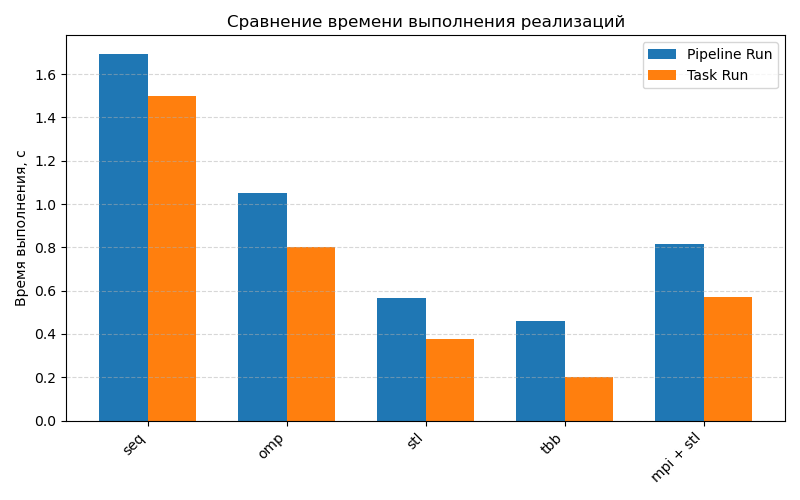
\includegraphics[height=8cm]{img/perf_stat_info_1.png}
\caption{\label{fig:visualClass} Результаты тестирования производительности реализаций}
\end{figure}

\begin{figure}[H]
\centering
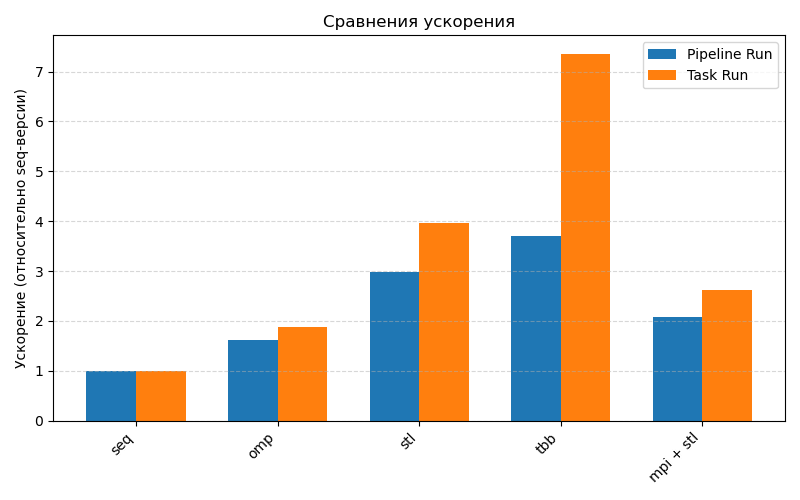
\includegraphics[height=8cm]{img/perf_stat_info_2.png}
\caption{\label{fig:visualClass} Относительное ускорение различных версий}
\end{figure}

\section{Анализ результатов}
Из анализа гистограмм можно сделать следующие выводы:

\begin{enumerate}
  \item \textbf{Последовательная реализация (seq)} ожидаемо демонстрирует наибольшее время выполнения и служит базовой точкой отсчёта для измерения ускорения.

  \item \textbf{OpenMP-реализация (omp)} показывает умеренное ускорение по сравнению с последовательной версией: ускорение составляет около 1.5--2 раз в зависимости от сценария (Pipeline Run / Task Run). Это указывает на эффективное, но не полное использование параллельных ресурсов.

  \item \textbf{STL-реализация (stl)} демонстрирует более высокое ускорение (до 4 раз в Task Run), что говорит о лучшей масштабируемости при использовании стандартных средств параллелизма C++.

  \item \textbf{TBB-реализация (tbb)} показывает наибольшее ускорение (более чем в 7 раз в Task Run), что свидетельствует о высокой эффективности библиотеки Intel TBB в данном контексте. При этом наблюдается заметная разница между Pipeline Run и Task Run, что может указывать на различия в характере нагрузки.

  \item \textbf{Комбинированная реализация (mpi + stl)} уступает TBB и STD-реализациям в эффективности, хотя и демонстрирует ускорение по сравнению с базовой версией. Это может быть связано с накладными расходами на коммуникацию в MPI.

\end{enumerate}

Наибольшего ускорения удалось достичь с помощью реализации на основе библиотеки TBB, особенно в режиме Task Run. Это подтверждает целесообразность использования высокоуровневых средств параллелизма при разработке производительных решений.

\subsection*{Причины различий в производительности}
\begin{enumerate}
  \item \textbf{Последовательная зависимость итераций.}  
    Алгоритм построения выпуклой оболочки по Джарвису является условно последовательным: выбор следующей вершины зависит от результата предыдущей итерации. Это ограничивает потенциальный уровень параллелизма и приводит к тому, что лишь часть работы может быть распараллелена без изменения самого алгоритма.
  
  \item \textbf{Накладные расходы на управление потоками и задачами.}  
    \begin{itemize}
      \item В \texttt{std::thread} и OpenMP каждый запуск цикла или фор-параллельная секция создаёт или синхронизирует большое число потоков, что даёт заметные расходы времени на создание/завершение потоков, блокировки и барьеры.  
      \item В MPI каждая collective-операция (\texttt{MPI\_Bcast}, \texttt{MPI\_Gather}, \texttt{MPI\_Scatterv}) требует сериализации/десериализации данных и межпроцессного обмена, что особенно дорого при большом размере массива точек \(n\).
    \end{itemize}

  \item \textbf{Коммуникационные накладные расходы MPI.}  
    При разбиении данных между процессами в MPI-версии значительную долю времени занимает передача массива точек и результатов кандидатов между процессами:
    \[
      T_{\rm comm} \sim \alpha + \beta \, n,
    \]
    где \(\alpha\) — латентность сети, \(\beta\) — стоимость передачи одного элемента. 

  \item \textbf{Стратегии балансировки нагрузки.}  
    \begin{itemize}
      \item В TBB используется динамическая балансировка (\emph{work stealing}), что позволяет равномернее распределять работу между потоками и снижает простой.  
      \item В OpenMP и STL-реализациях разбиение на фиксированные чанки может приводить к неравномерной загрузке при неравномерном распределении точек.
    \end{itemize}

  \item \textbf{Локальность данных и кэширование.}  
    Распараллеленные версии, перескакивая по разным участкам массива, хуже используют кэш-память процессора. Библиотека TBB, благодаря мелким блокам и итеративным диапазонам, чаще работает с «горячими» участками данных, что усиливает выигрыш в производительности.

  \item \textbf{Накладные расходы на вспомогательные структуры данных.}  
    Использование в MPI \texttt{MPI\_Datatype}, в STL — \texttt{std::unordered\_set}, в TBB — \texttt{tbb::concurrent\_unordered\_set} и \texttt{tbb::concurrent\_vector} добавляет дополнительную нагрузку на построение, синхронизацию и управление памятью.
\end{enumerate}

Таким образом, наибольшее ускорение в TBB-версии объясняется сочетанием эффективного пула потоков, динамической балансировки задач и оптимизированных concurrent-контейнеров, тогда как MPI и чисто потоковые реализации несут существенные накладные расходы на коммуникацию и синхронизацию.

\section{Выводы}
В рамках данной лабораторной работы была разработана и экспериментально оценена эффективность метода построения выпуклой оболочки по Джарвису (Gift Wrapping) на наборе из \(N\) точек. Были реализованы и сравнены следующие параллельные модели:
\begin{itemize}
  \item \emph{TBB} (Intel Threading Building Blocks) с динамической балансировкой задач;
  \item \emph{STL-pool} (пул потоков на базе \texttt{std::thread});
  \item \emph{OpenMP} с директивой \texttt{\#pragma omp parallel for};
  \item \emph{MPI+STL} (гибридный подход с распределением по процессам и внутренним пулом потоков).
\end{itemize}

Сравнение относительного ускорения (см. Рис.~2) позволило установить следующий порядок по убыванию производительности:
\[
\mathrm{TBB} \;>\; \mathrm{STL\mbox{-}pool} \;>\; \mathrm{MPI+STL} \;>\; \mathrm{OpenMP}\,.
\]
Максимальный прирост (до \(7\times\) в режиме Task Run) обеспечен реализацией на TBB благодаря динамическому распределению задач и оптимизированным concurrent‐контейнерам. Реализация на STL демонстрирует стабильный ускоренный режим (\(2\!-\!4\times\)), а гибридный MPI+STL испытывает накладные расходы на коммуникацию. Наименее эффективной оказалась OpenMP-версия из-за статического разбиения и затрат на синхронизацию.

В ходе данной лабораторной работы было выявлено, что для алгоритма со строгой последовательной зависимостью итераций (на примере метода Джарвиса) ключевым фактором ускорения является адаптивная балансировка нагрузки и минимизация синхронизационных издержек.
\newpage
\section*{Список литературы}

\begin{enumerate}
    \item Сысоев А.В., Мееров И.Б., Сиднев А.А. \textit{Средства разработки параллельных программ для систем с общей памятью. Библиотека Intel Threading Building Blocks}. — Нижний Новгород, 2007.
  \item James Reinders, \emph{Intel Threading Building Blocks: Outfitting C++ for Multi-Core Processor Parallelism}, O’Reilly Media, 2007.
  \item Pascal Pacheco, \emph{Parallel Programming with Intel Threading Building Blocks}, Manning, 2011.
  \item William Gropp, Ewing Lusk, Anthony Skjellum, \emph{Using MPI: Portable Parallel Programming with the Message-Passing Interface}, MIT Press, 1999.
  \item Michael Snir, Steve Otto, Steven Huss-Lewis, David Walker, Jack Dongarra, \emph{MPI: The Complete Reference}, MIT Press, 1998.
  \item Anthony Williams, \emph{C++ Concurrency in Action: Practical Multithreading}, Manning, 2012.
  \item Hans-J. Boehm, Sarita Adve, “Foundations of the C++ Concurrency Memory Model”, в \emph{Proceedings of the 2004 ACM SIGPLAN Conference on Programming Language Design and Implementation}, 2004.
  \item Barbara Chapman, Gabriele Jost, Ruud van der Pas, Frances Seidel, \emph{Using OpenMP: Portable Shared Memory Parallel Programming}, MIT Press, 2001.
  \item OpenMP Architecture Review Board, \emph{OpenMP Application Program Interface Version 5.2}, 2024.
  \item R. A. Jarvis, “On the identification of the convex hull of a finite set of points in the plane”, \emph{Information Processing Letters}, vol.~2, no.~1, pp.~18–21, 1973.
  \item Franco P. Preparata, Michael Ian Shamos, \emph{Computational Geometry: An Introduction}, Springer, 1985.
\end{enumerate}
\newpage
\section{Приложение}
\begin{lstlisting}[caption={SEQ-версия алгоритма}]
int shulpin_i_jarvis_seq::JarvisSequential::Orientation(const Point& p, const Point& q, const Point& r) {
  double val = ((q.y - p.y) * (r.x - q.x)) - ((q.x - p.x) * (r.y - q.y));
  if (std::fabs(val) < 1e-9) {
    return 0;
  }
  return (val > 0) ? 1 : 2;
}

void shulpin_i_jarvis_seq::JarvisSequential::MakeJarvisPassage(std::vector<shulpin_i_jarvis_seq::Point>& input_jar, std::vector<shulpin_i_jarvis_seq::Point>& output_jar) {
  size_t total = input_jar.size();
  output_jar.clear();
  // clang-format off
  std::unordered_set<shulpin_i_jarvis_seq::Point, 
                     shulpin_i_jarvis_seq::PointHash, 
                     shulpin_i_jarvis_seq::PointEqual> unique_points;
  // clang-format on
  size_t start = 0;
  for (size_t i = 1; i < total; ++i) {
    if (input_jar[i].x < input_jar[start].x ||
        (input_jar[i].x == input_jar[start].x && input_jar[i].y < input_jar[start].y)) {
      start = i;
    }
  }

  size_t active = start;
  do {
    const auto& current = input_jar[active];
    if (unique_points.find(current) == unique_points.end()) {
      output_jar.emplace_back(current);
      unique_points.insert(current);
    }

    size_t candidate = (active + 1) % total;
    for (size_t index = 0; index < total; ++index) {
      if (index == active) {
        continue;
      }

      if (Orientation(input_jar[active], input_jar[index], input_jar[candidate]) == 2) {
        candidate = index;
      }
    }

    active = candidate;
  } while (active != start);
}
\end{lstlisting}

\begin{lstlisting}[caption={OMP-версия алгоритма}]
namespace {
int Orientation(const shulpin_i_jarvis_omp::Point& p, const shulpin_i_jarvis_omp::Point& q,
                const shulpin_i_jarvis_omp::Point& r) {
  double val = ((q.y - p.y) * (r.x - q.x)) - ((q.x - p.x) * (r.y - q.y));
  if (std::fabs(val) < 1e-9) {
    return 0;
  }
  return (val > 0) ? 1 : 2;
}
}  // namespace

void shulpin_i_jarvis_omp::JarvisOMPParallel::MakeJarvisPassageOMP(
    std::vector<shulpin_i_jarvis_omp::Point>& input_jar, std::vector<shulpin_i_jarvis_omp::Point>& output_jar) {
  int total = static_cast<int>(input_jar.size());
  output_jar.clear();

  std::unordered_set<shulpin_i_jarvis_omp::Point, shulpin_i_jarvis_omp::PointHash, shulpin_i_jarvis_omp::PointEqual> unique_points;
  std::vector<shulpin_i_jarvis_omp::Point> hull;
  hull.reserve(total);

  int start = 0;
  for (int i = 1; i < total; ++i) {
    const auto& a = input_jar[i];
    const auto& b = input_jar[start];
    if (a.x < b.x || (a.x == b.x && a.y < b.y)) {
      start = i;
    }
  }
  int active = start;

  do {
    const Point& current = input_jar[active];
    if (unique_points.find(current) == unique_points.end()) {
      hull.push_back(current);
      unique_points.insert(current);
    }

    int candidate = (active + 1) % total;
    std::vector<int> thread_candidates(omp_get_max_threads(), candidate);

#pragma omp parallel
    {
      int tid = omp_get_thread_num();
      int local_candidate = candidate;

#pragma omp for nowait
      for (int i = 0; i < total; ++i) {
        if (i == active) continue;
        if (Orientation(current, input_jar[i], input_jar[local_candidate]) == 2) {
          local_candidate = i;
        }
      }

      thread_candidates[tid] = local_candidate;
    }

    for (int tid = 0; tid < static_cast<int>(thread_candidates.size()); ++tid) {
      int cand = thread_candidates[tid];
      if (Orientation(current, input_jar[cand], input_jar[candidate]) == 2) {
        candidate = cand;
      }
    }

    if (candidate == active) {
      break;
    }

    active = candidate;

  } while (active != start);

  output_jar = std::move(hull);
}
\end{lstlisting}\begin{lstlisting}[caption={TBB-версия алгоритма}]
namespace {
int Orientation(const shulpin_i_jarvis_tbb::Point& p, const shulpin_i_jarvis_tbb::Point& q,
                const shulpin_i_jarvis_tbb::Point& r) {
  double val = ((q.y - p.y) * (r.x - q.x)) - ((q.x - p.x) * (r.y - q.y));
  if (std::fabs(val) < 1e-9) {
    return 0;
  }
  return (val > 0) ? 1 : 2;
}
}  // namespace

void shulpin_i_jarvis_tbb::JarvisTBBParallel::MakeJarvisPassageTBB(
    std::vector<shulpin_i_jarvis_tbb::Point>& input_jar, std::vector<shulpin_i_jarvis_tbb::Point>& output_jar) {
  int n = static_cast<int>(input_jar.size());

  int start = 0;
  for (int i = 1; i < n; ++i) {
    if (input_jar[i].x < input_jar[start].x ||
        (input_jar[i].x == input_jar[start].x && input_jar[i].y < input_jar[start].y)) {
      start = i;
    }
  }

  std::vector<Point> hull;
  hull.reserve(n);
  tbb::concurrent_unordered_set<Point, PointHash, PointEqual> visited;

  int current = start;
  do {
    const Point& cur_pt = input_jar[current];
    if (visited.insert(cur_pt).second) {
      hull.push_back(cur_pt);
    }

    struct BlockCandidate {
      int index;
      Point pt;
    };
    tbb::concurrent_vector<BlockCandidate> local_cands;
    int initial = (current + 1) % n;

    tbb::parallel_for(tbb::blocked_range<int>(0, n), [&](const tbb::blocked_range<int>& r) {
      int best = initial;
      for (int i = r.begin(); i < r.end(); ++i) {
        if (i == current) {
          continue;
        }
        int orient = Orientation(cur_pt, input_jar[i], input_jar[best]);
        if (orient == 2) {
          best = i;
        }
      }
      local_cands.push_back({best, input_jar[best]});
    });

    int candidate = local_cands[0].index;
    for (size_t i = 1; i < local_cands.size(); ++i) {
      int idx = local_cands[i].index;
      int orient = Orientation(cur_pt, input_jar[idx], input_jar[candidate]);
      if (orient == 2) {
        candidate = idx;
      }
    }

    current = candidate;
  } while (current != start);

  output_jar = std::move(hull);
}
\end{lstlisting}
\begin{lstlisting}[caption={STL-версия алгоритма}]
#ifdef __linux__
// NOLINTBEGIN
void shulpin_i_jarvis_stl::JarvisSTLParallel::MakeJarvisPassageSTL(
    std::vector<shulpin_i_jarvis_stl::Point>& input_jar, std::vector<shulpin_i_jarvis_stl::Point>& output_jar) {
  output_jar.clear();

  std::unordered_set<Point, PointHash, PointEqual> unique_points;

  size_t most_left = 0;
  for (size_t i = 1; i < input_jar.size(); ++i) {
    if (input_jar[i].x < input_jar[most_left].x ||
        (input_jar[i].x == input_jar[most_left].x && input_jar[i].y < input_jar[most_left].y)) {
      most_left = i;
    }
  }

  const Point& min_point = input_jar[most_left];
  std::vector<Point> convex_hull = {min_point};
  Point prev_point = min_point;
  Point next_point;

  int num_threads = ppc::util::GetPPCNumThreads();
  int chunk_size = static_cast<int>(input_jar.size() / num_threads);

  std::vector<std::thread> threads;
  std::vector<Point> candidates(num_threads, input_jar[0]);
  std::vector<bool> thread_ready(num_threads, false);
  std::vector<bool> thread_done(num_threads, false);
  std::mutex mtx;
  std::condition_variable cv;
  bool stop = false;

  auto findNextPointThread = [&](int tid) {
    while (true) {
      std::unique_lock<std::mutex> lock(mtx);
      cv.wait(lock, [&] { return thread_ready[tid] || stop; });

      if (stop) {
        return;
      }

      int start = tid * chunk_size;
      int end = (tid == num_threads - 1) ? static_cast<int>(input_jar.size()) : (tid + 1) * chunk_size;
      Point candidate = input_jar[start];

      for (int i = start; i < end; ++i) {
        const auto& point = input_jar[i];
        if (point == prev_point) {
          continue;
        }

        double cross_product = ((point.y - prev_point.y) * (candidate.x - prev_point.x)) -
                               ((point.x - prev_point.x) * (candidate.y - prev_point.y));
        double dist1 = std::pow(point.x - prev_point.x, 2) + std::pow(point.y - prev_point.y, 2);
        double dist2 = std::pow(candidate.x - prev_point.x, 2) + std::pow(candidate.y - prev_point.y, 2);

        if (cross_product > 0 || (cross_product == 0 && dist1 > dist2)) {
          candidate = point;
        }
      }

      candidates[tid] = candidate;
      thread_ready[tid] = false;
      thread_done[tid] = true;
      cv.notify_all();
    }
  };

  for (int i = 0; i < num_threads; ++i) {
    threads.emplace_back(findNextPointThread, i);
  }

  do {
    next_point = input_jar[0];

    {
      std::unique_lock<std::mutex> lock(mtx);
      for (int i = 0; i < num_threads; ++i) {
        thread_ready[i] = true;
        thread_done[i] = false;
      }
    }
    cv.notify_all();

    {
      std::unique_lock<std::mutex> lock(mtx);
      cv.wait(lock, [&] {
        return std::ranges::all_of(thread_done.begin(), thread_done.end(), [](bool done) { return done; });
      });
    }

    for (const auto& candidate : candidates) {
      double cross_product = ((candidate.y - prev_point.y) * (next_point.x - prev_point.x)) -
                             ((candidate.x - prev_point.x) * (next_point.y - prev_point.y));
      double dist1 = std::pow(candidate.x - prev_point.x, 2) + std::pow(candidate.y - prev_point.y, 2);
      double dist2 = std::pow(next_point.x - prev_point.x, 2) + std::pow(next_point.y - prev_point.y, 2);
      if (cross_product > 0 || (cross_product == 0 && dist1 > dist2)) {
        next_point = candidate;
      }
    }

    if (unique_points.find(next_point) == unique_points.end()) {
      output_jar.push_back(next_point);
      unique_points.insert(next_point);
    }

    prev_point = next_point;

  } while (next_point != min_point);

  {
    std::unique_lock<std::mutex> lock(mtx);
    stop = true;
    cv.notify_all();
  }

  for (auto& thread : threads) {
    if (thread.joinable()) {
      thread.join();
    }
  }
}
// NOLINTEND
#else
void shulpin_i_jarvis_stl::JarvisSTLParallel::MakeJarvisPassageSTL(
    std::vector<shulpin_i_jarvis_stl::Point>& input_jar, std::vector<shulpin_i_jarvis_stl::Point>& output_jar) {
  output_jar.clear();

  std::unordered_set<shulpin_i_jarvis_stl::Point, shulpin_i_jarvis_stl::PointHash, shulpin_i_jarvis_stl::PointEqual>
      unique_points;

  size_t most_left = 0;
  for (size_t i = 1; i < input_jar.size(); ++i) {
    if (input_jar[i].x < input_jar[most_left].x ||
        (input_jar[i].x == input_jar[most_left].x && input_jar[i].y < input_jar[most_left].y)) {
      most_left = i;
    }
  }

  const Point& min_point = input_jar[most_left];
  std::vector<Point> convex_hull = {min_point};
  Point prev_point = min_point;
  Point next_point;

  auto findNextPoint = [](const Point& current_point, const std::vector<Point>& points, int start, int end,
                          Point& candidate) {
    for (int i = start; i < end; ++i) {
      const auto& point = points[i];
      if (point == current_point) {
        continue;
      }
      double cross_product = ((point.y - current_point.y) * (candidate.x - current_point.x)) -
                             ((point.x - current_point.x) * (candidate.y - current_point.y));
      double dist_current_point = std::pow(point.x - current_point.x, 2) + std::pow(point.y - current_point.y, 2);
      double dist_candidate = std::pow(candidate.x - current_point.x, 2) + std::pow(candidate.y - current_point.y, 2);
      if (cross_product > 0 || (cross_product == 0 && dist_current_point > dist_candidate)) {
        candidate = point;
      }
    }
  };

  do {
    next_point = input_jar[0];
    int num_threads = ppc::util::GetPPCNumThreads();
    int chunk_size = input_jar.size() / num_threads;
    std::vector<std::thread> threads;
    std::vector<Point> candidates(num_threads, next_point);

    for (int i = 0; i < num_threads; ++i) {
      int start = i * chunk_size;
      int end = (i == num_threads - 1) ? input_jar.size() : (i + 1) * chunk_size;
      threads.emplace_back(findNextPoint, std::ref(prev_point), std::cref(input_jar), start, end,
                           std::ref(candidates[i]));
    }

    for (auto& thread : threads) {
      if (thread.joinable()) thread.join();
    }

    for (const auto& candidate : candidates) {
      double cross_product = ((candidate.y - prev_point.y) * (next_point.x - prev_point.x)) -
                             ((candidate.x - prev_point.x) * (next_point.y - prev_point.y));
      double dist_prev_point = std::pow(candidate.x - prev_point.x, 2) + std::pow(candidate.y - prev_point.y, 2);
      double dist_next_point = std::pow(next_point.x - prev_point.x, 2) + std::pow(next_point.y - prev_point.y, 2);
      if (cross_product > 0 || (cross_product == 0 && dist_prev_point > dist_next_point)) {
        next_point = candidate;
      }
    }

    if (unique_points.find(next_point) == unique_points.end()) {
      output_jar.push_back(next_point);
      unique_points.insert(next_point);
    }

    prev_point = next_point;

  } while (next_point != min_point);
}
#endif
\end{lstlisting}
\begin{lstlisting}[caption={Гибридная версия алгоритма(MPI+STL)}]
namespace {
shulpin_i_jarvis_all::Point FindLocalCandidate(const shulpin_i_jarvis_all::Point& current,
                                               const std::vector<shulpin_i_jarvis_all::Point>& points,
                                               int num_threads) {
shulpin_i_jarvis_all::Point FindLocalCandidate(const shulpin_i_jarvis_all::Point& current,
                                               const std::vector<shulpin_i_jarvis_all::Point>& points,
                                               int num_threads) {
  std::vector<shulpin_i_jarvis_all::Point> local_cand(num_threads);

  auto worker = [&](int tid) {
    size_t chunk = points.size() / num_threads;
    size_t start = tid * chunk;
    size_t end = (tid == num_threads - 1 ? points.size() : start + chunk);

    shulpin_i_jarvis_all::Point candidate;
    if (start < end) {
      candidate = points[start];
      for (size_t i = start; i < end; ++i) {
        const auto& p = points[i];
        if (p == current) {
          continue;
        }
        double cross =
            ((p.y - current.y) * (candidate.x - current.x)) - ((p.x - current.x) * (candidate.y - current.y));
        double d_p = std::pow(p.x - current.x, 2) + std::pow(p.y - current.y, 2);
        double d_c = std::pow(candidate.x - current.x, 2) + std::pow(candidate.y - current.y, 2);
        if (cross > 0 || (cross == 0 && d_p > d_c)) {
          candidate = p;
        }
      }
    } else {
      candidate = current;
    }

    local_cand[tid] = candidate;
  };

  std::vector<std::thread> threads;
  threads.reserve(num_threads);
  for (int t = 0; t < num_threads; ++t) {
    threads.emplace_back(worker, t);
  }
  for (auto& th : threads) {
    th.join();
  }

  shulpin_i_jarvis_all::Point best = local_cand[0];
  for (int t = 1; t < num_threads; ++t) {
    const auto& cand = local_cand[t];
    double cross = ((cand.y - current.y) * (best.x - current.x)) - ((cand.x - current.x) * (best.y - current.y));
    double d_c = std::pow(cand.x - current.x, 2) + std::pow(cand.y - current.y, 2);
    double d_b = std::pow(best.x - current.x, 2) + std::pow(best.y - current.y, 2);
    if (cross > 0 || (cross == 0 && d_c > d_b)) {
      best = cand;
    }
  }
  return best;
}


}  // namespace

// NOLINTNEXTLINE(readability-function-cognitive-complexity, readability-make-member-function-const)
void shulpin_i_jarvis_all::JarvisALLParallel::MakeJarvisPassageALL(
    std::vector<shulpin_i_jarvis_all::Point>& input_jar, std::vector<shulpin_i_jarvis_all::Point>& output_jar) {
  output_jar.clear();

  MPI_Datatype mpi_point = MPI_DATATYPE_NULL;
  MPI_Type_contiguous(2, MPI_DOUBLE, &mpi_point);
  MPI_Type_commit(&mpi_point);

  size_t n = input_jar.size();
  MPI_Bcast(&n, 1, MPI_UNSIGNED_LONG, 0, MPI_COMM_WORLD);

  if (rank_ != 0) {
    input_jar.resize(n);
  }

  MPI_Bcast(input_jar.data(), static_cast<int>(n), mpi_point, 0, MPI_COMM_WORLD);

  size_t most_left = 0;
  if (rank_ == 0) {
    for (size_t i = 1; i < n; ++i) {
      if (input_jar[i].x < input_jar[most_left].x ||
          (input_jar[i].x == input_jar[most_left].x && input_jar[i].y < input_jar[most_left].y)) {
        most_left = i;
      }
    }
  }
  MPI_Bcast(&most_left, 1, MPI_UNSIGNED_LONG, 0, MPI_COMM_WORLD);
  Point min_point = input_jar[most_left];

  std::vector<int> counts(world_size_);
  std::vector<int> displs(world_size_);
  int base = static_cast<int>(n / world_size_);
  int rem = static_cast<int>(n % world_size_);
  int offset = 0;
  for (int i = 0; i < world_size_; ++i) {
    counts[i] = base + (i < rem ? 1 : 0);
    displs[i] = offset;
    offset += counts[i];
  }

  std::vector<Point> local_points(counts[rank_]);
  MPI_Scatterv(input_jar.data(), counts.data(), displs.data(), mpi_point, local_points.data(), counts[rank_], mpi_point,
               0, MPI_COMM_WORLD);

  std::unordered_set<Point, PointHash, PointEqual> unique_points;
  if (rank_ == 0) {
    output_jar.push_back(min_point);
    unique_points.insert(min_point);
  }

  Point prev_point = min_point;
  Point next_point;
  int num_threads = ppc::util::GetPPCNumThreads();

  bool done = false;

  do {
    MPI_Bcast(&prev_point, 1, mpi_point, 0, MPI_COMM_WORLD);

    Point local_candidate = FindLocalCandidate(prev_point, local_points, num_threads);

    std::vector<Point> all_cand;
    if (rank_ == 0) {
      all_cand.resize(world_size_);
    }
    MPI_Gather(&local_candidate, 1, mpi_point, all_cand.data(), 1, mpi_point, 0, MPI_COMM_WORLD);

    if (rank_ == 0) {
      next_point = all_cand[0];
      for (int i = 1; i < world_size_; ++i) {
        const auto& cand = all_cand[i];
        double cross = ((cand.y - prev_point.y) * (next_point.x - prev_point.x)) -
                       ((cand.x - prev_point.x) * (next_point.y - prev_point.y));
        double d_c = std::pow(cand.x - prev_point.x, 2) + std::pow(cand.y - prev_point.y, 2);
        double d_n = std::pow(next_point.x - prev_point.x, 2) + std::pow(next_point.y - prev_point.y, 2);
        if (cross > 0 || (cross == 0 && d_c > d_n)) {
          next_point = cand;
        }
      }

      done = (next_point == min_point);

      if (!done && unique_points.find(next_point) == unique_points.end()) {
        output_jar.push_back(next_point);
        unique_points.insert(next_point);
      }
    }

    MPI_Bcast(&next_point, 1, mpi_point, 0, MPI_COMM_WORLD);
    MPI_Bcast(&done, 1, MPI_C_BOOL, 0, MPI_COMM_WORLD);

    prev_point = next_point;

  } while (!done);

  MPI_Type_free(&mpi_point);
}
\end{lstlisting}
\end{document}